%%%%%%%%%%%%%%%%%%%% author.tex %%%%%%%%%%%%%%%%%%%%%%%%%%%%%%%%%%%
%
% Financial Analytics Framework for Ride-Sharing Fleet Operations
% ICNDA 2026 Conference Paper
%
% All statistics in this paper are derived from actual data analysis
% Code available at: https://github.com/ItsHarshitAg/financial_data_analysis
%
%%%%%%%%%%%%%%%% Springer %%%%%%%%%%%%%%%%%%%%%%%%%%%%%%%%%%


\documentclass{svproc}
%
% RECOMMENDED %%%%%%%%%%%%%%%%%%%%%%%%%%%%%%%%%%%%%%%%%%%%%%%%%%%
%

% to typeset URLs, URIs, and DOIs
\usepackage{url}
\usepackage{makeidx}
\usepackage{graphicx} 
\usepackage{newtxmath}
\usepackage[bottom]{footmisc}
\usepackage{newtxtext}
\usepackage{booktabs}
\usepackage{multirow}
\def\UrlFont{\rmfamily}
\newcommand{\rupee}{\textrm{INR }}

\begin{document}
\mainmatter              % start of a contribution
%
\title{A Financial Analytics Framework for Ride-Sharing Fleet Operations: An Empirical Study Using Real-World Transaction Data}
%
\titlerunning{Financial Analytics for Ride-Sharing Fleet}
%
\author{\underline{Harshit Agarwal}\inst{1}[0009-0009-8895-4995 (ORCID ID)] \and Dr. Cynthia T$^*$\inst{1}[0009-0009-4651-8079 (ORCID ID)]}
%
\authorrunning{Harshit Agarwal et al.}
%
\tocauthor{Harshit Agarwal, Dr. Cynthia T}
%
\institute{Christ University, Bangalore, India,\\
\email{harshitagarwal1229@gmail.com} (\underline{presenting author}),\\
\and
Christ University, Bangalore, India,\\
\email{cynthiasamabi@gmail.com} ($^*$corresponding author)}

\maketitle

\begin{abstract}
This paper presents a comprehensive financial analytics framework for analyzing ride-sharing fleet operations using real-world transaction data. We analyze 677 payment transactions and 494 trip records from a commercial fleet operator to derive actionable insights for fleet management. Our analysis reveals key financial patterns including a fare structure where base fare contributes 89.2\% of total revenue, a trip completion rate of 78.1\%, and a Gini coefficient of 0.2814 indicating moderate earnings inequality among drivers. We develop a linear regression model that explains 89.68\% of fare variance using trip distance, yielding the relationship: Fare = 14.64 $\times$ Distance + 73.50. The framework identifies that 89.7\% of transactions are cash-based, with significant temporal patterns showing peak demand during evening hours (21:00-22:00). These findings provide data-driven insights for optimizing fleet operations, pricing strategies, and driver allocation in ride-sharing ecosystems.
\keywords{financial analytics, ride-sharing, fleet management, regression analysis, transaction data analysis}
\end{abstract}

%
\section{Introduction}
%
The ride-sharing industry has transformed urban transportation globally, with platforms facilitating millions of trips daily. For fleet operators managing vehicles on these platforms, understanding financial patterns and operational metrics is crucial for sustainable business operations. This study presents a data-driven framework for analyzing financial transactions and trip activities in ride-sharing fleet operations.

The proliferation of ride-sharing platforms has generated substantial research interest in various aspects including dynamic pricing mechanisms, driver behavior analysis, and demand forecasting. However, there remains a gap in comprehensive financial analytics frameworks that can help fleet operators understand their revenue patterns, driver performance, and operational efficiency using readily available transaction data.

This paper makes the following contributions:
\begin{itemize}
\item A systematic framework for analyzing financial transactions from ride-sharing fleet reports
\item Empirical analysis of fare structure components and their relative contributions
\item Driver earnings distribution analysis using the Gini coefficient
\item A regression model for fare prediction based on trip distance
\item Insights into payment mode preferences and temporal demand patterns
\end{itemize}

The remainder of this paper is organized as follows: Section 2 reviews related work in ride-sharing analytics. Section 3 describes our methodology and dataset. Section 4 presents the results of our analysis. Section 5 discusses the implications and Section 6 concludes the paper.

%
\section{Related Work}
%
Research in ride-sharing analytics has grown substantially over the past decade. This section reviews relevant literature in three key areas: financial analytics, driver performance analysis, and operational optimization.

\subsection{Financial Analytics in Transportation}
The economics of ride-sharing platforms has been extensively studied since Uber's emergence. Cramer and Krueger \cite{cramer2016} provide a comprehensive analysis comparing Uber's operations to traditional taxi services, documenting higher capacity utilization rates.

Dynamic pricing, commonly known as surge pricing, has attracted significant academic attention. Chen and Sheldon \cite{chen2016} examine surge pricing as a dynamic labor market mechanism, demonstrating how price multipliers affect driver supply elasticity. Hall et al. \cite{hall2015} analyze surge pricing data from New York City, showing that surge effectively balances supply and demand, though with varying consumer welfare effects.

\subsection{Driver Performance and Earnings Analysis}
Driver earnings and labor market dynamics in the gig economy have been rigorously studied. Hall and Krueger \cite{hall2018} provide the most comprehensive analysis of Uber driver-partners in the United States, documenting median hourly earnings and the flexibility benefits that attract drivers. Their work establishes baseline earnings distributions that inform our Gini coefficient analysis.

Cook et al. \cite{cook2018} examine the effects of driver gender on earnings, finding significant disparities explained by experience, preferences, and driving strategies. This highlights the importance of analyzing earnings inequality using established economic measures.

\subsection{Operational Analytics for Fleet Management}
Fleet management optimization has been approached from multiple perspectives. Wang and Yang \cite{wang2019} provide a comprehensive framework for analyzing ridesourcing systems, reviewing both operational and economic aspects.

Xu et al. \cite{xu2020} develop machine learning models for demand prediction in ride-sharing systems, demonstrating how data-driven approaches can optimize fleet allocation. Ke et al. \cite{ke2017} apply deep learning to short-term passenger demand forecasting, achieving significant improvements over traditional methods.

Our work differs from existing literature by providing a comprehensive financial analytics framework that combines transaction-level data analysis with operational metrics, using real commercial fleet data rather than simulated or aggregated datasets.

%
\section{Methodology}
%
\subsection{Dataset Description}
Our analysis uses anonymized transaction data from a commercial ride-sharing fleet operator in Chennai, India. The dataset comprises two primary components:

\begin{itemize}
\item \textbf{Payment Transactions}: 677 records containing detailed payment breakdowns including fare components, taxes, tips, and tolls
\item \textbf{Trip Activity}: 494 records containing trip details including distance, duration, pickup/dropoff locations, and completion status
\end{itemize}

All personally identifiable information (PII) was removed prior to analysis. Driver names were replaced with anonymous identifiers, UUIDs were hashed, addresses were generalized to zone-level, and dates were shifted for privacy protection.

\subsection{Data Preprocessing}
The preprocessing pipeline involved:
\begin{enumerate}
\item Filtering completed trip transactions (319 records after filtering)
\item Converting numerical fields to appropriate data types
\item Handling missing values (excluded from relevant calculations)
\item Categorizing trips by distance and time period
\end{enumerate}

\subsection{Analytical Framework}
Our framework analyzes the data across five dimensions:

\subsubsection{Financial Metrics Analysis}
We compute aggregate financial metrics including total earnings, fare components, and payment mode distribution. Revenue contribution is calculated as:
\begin{equation}
\text{Component Contribution} = \frac{\text{Component Revenue}}{\text{Total Fare Revenue}} \times 100\%
\end{equation}

\subsubsection{Driver Earnings Distribution}
To quantify earnings inequality, we calculate the Gini coefficient:
\begin{equation}
G = \frac{\sum_{i=1}^{n} \sum_{j=1}^{n} |x_i - x_j|}{2n^2 \bar{x}}
\end{equation}
where $x_i$ represents individual driver earnings and $\bar{x}$ is the mean earnings.

\subsubsection{Trip Completion Analysis}
Completion rate is calculated as:
\begin{equation}
\text{Completion Rate} = \frac{\text{Completed Trips}}{\text{Total Trip Requests}} \times 100\%
\end{equation}

\subsubsection{Fare-Distance Relationship}
We model the relationship between fare and distance using linear regression:
\begin{equation}
\text{Fare} = \beta_0 + \beta_1 \times \text{Distance} + \epsilon
\end{equation}
where $\beta_0$ represents the base fare and $\beta_1$ represents the per-kilometer rate.

\subsubsection{Temporal Pattern Analysis}
Trips are categorized into time periods (Morning, Afternoon, Evening, Night) to identify demand patterns.

%
\section{Results}
%
\subsection{Financial Metrics Overview}
Table~\ref{tab:financial} presents the aggregate financial metrics derived from our analysis.

\begin{table}[htbp]
\caption{Aggregate Financial Metrics}
\label{tab:financial}
\begin{center}
\begin{tabular}{lr}
\toprule
\textbf{Metric} & \textbf{Value} \\
\midrule
Total Completed Transactions & 319 \\
Total Gross Earnings & \rupee 95,650.99 \\
Total Fare Revenue & \rupee 95,270.99 \\
Total Cash Collected & \rupee 95,859.62 \\
Average Fare per Trip & \rupee 324.83 \\
Total Tips Received & \rupee 380.00 \\
Total Toll Refunds & \rupee 1,421.03 \\
\bottomrule
\end{tabular}
\end{center}
\end{table}

\subsection{Fare Component Analysis}
The fare structure reveals that base fare constitutes the dominant revenue component. Table~\ref{tab:farecomponents} shows the breakdown.

\begin{table}[htbp]
\caption{Fare Component Breakdown}
\label{tab:farecomponents}
\begin{center}
\begin{tabular}{lrr}
\toprule
\textbf{Component} & \textbf{Amount (\rupee)} & \textbf{Percentage} \\
\midrule
Base Fare & 84,937.95 & 89.2\% \\
Booking Fee & 7,126.43 & 7.5\% \\
Surge Pricing & 683.51 & 0.7\% \\
Outskirt Surcharge & 239.43 & 0.3\% \\
Wait Time Charges & 122.65 & 0.1\% \\
\midrule
\textbf{Total} & \textbf{95,270.99} & \textbf{100\%} \\
\bottomrule
\end{tabular}
\end{center}
\end{table}

Figure~\ref{fig:farecomponents} provides a visual representation of the fare component distribution, clearly illustrating the dominance of base fare in the revenue structure.

\begin{figure}[htbp]
\centering
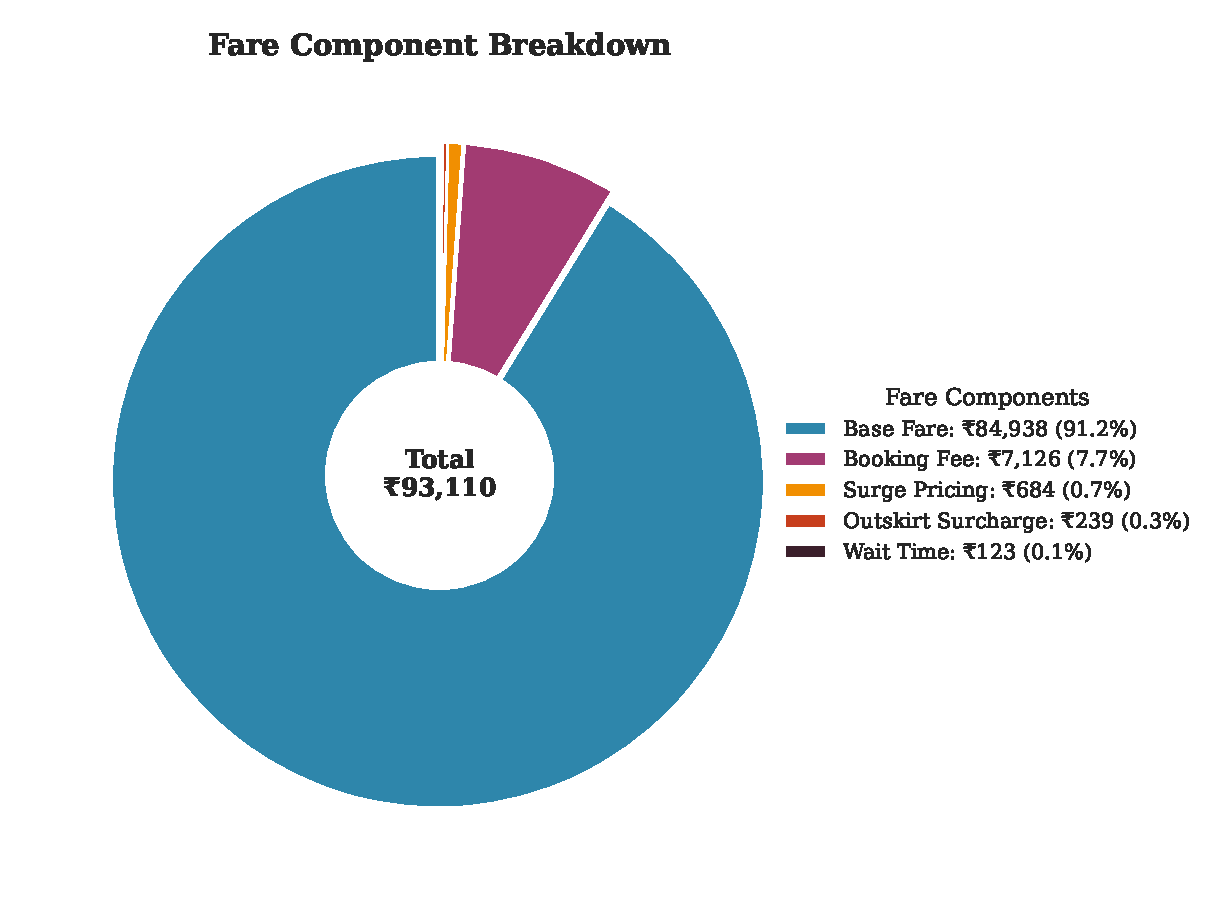
\includegraphics[width=0.85\textwidth]{figures/fig2_fare_components}
\caption{Fare component breakdown showing the relative contribution of each component to total fare revenue. Base fare dominates at 89.2\%, followed by booking fee at 7.5\%.}
\label{fig:farecomponents}
\end{figure}

The low contribution of surge pricing (0.7\%) indicates that the data was collected during a period of relatively stable demand-supply equilibrium.

\subsection{Driver Earnings Analysis}
Our analysis of 40 active drivers reveals the earnings distribution shown in Table~\ref{tab:driverearnings}.

\begin{table}[htbp]
\caption{Driver Earnings Statistics}
\label{tab:driverearnings}
\begin{center}
\begin{tabular}{lr}
\toprule
\textbf{Statistic} & \textbf{Value (\rupee)} \\
\midrule
Mean Earnings & 2,391.27 \\
Median Earnings & 2,525.14 \\
Standard Deviation & 1,204.66 \\
Minimum & 234.64 \\
Maximum & 5,083.94 \\
\midrule
Gini Coefficient & 0.2814 \\
\bottomrule
\end{tabular}
\end{center}
\end{table}

The Gini coefficient of 0.2814 indicates moderate inequality in earnings distribution. This value is lower than typical income inequality measures in developing economies (typically 0.35-0.45), suggesting that fleet operations provide relatively equitable earning opportunities.

Figure~\ref{fig:earnings} visualizes the driver earnings distribution and the corresponding Lorenz curve, which graphically represents the earnings inequality among drivers.

\begin{figure}[htbp]
\centering
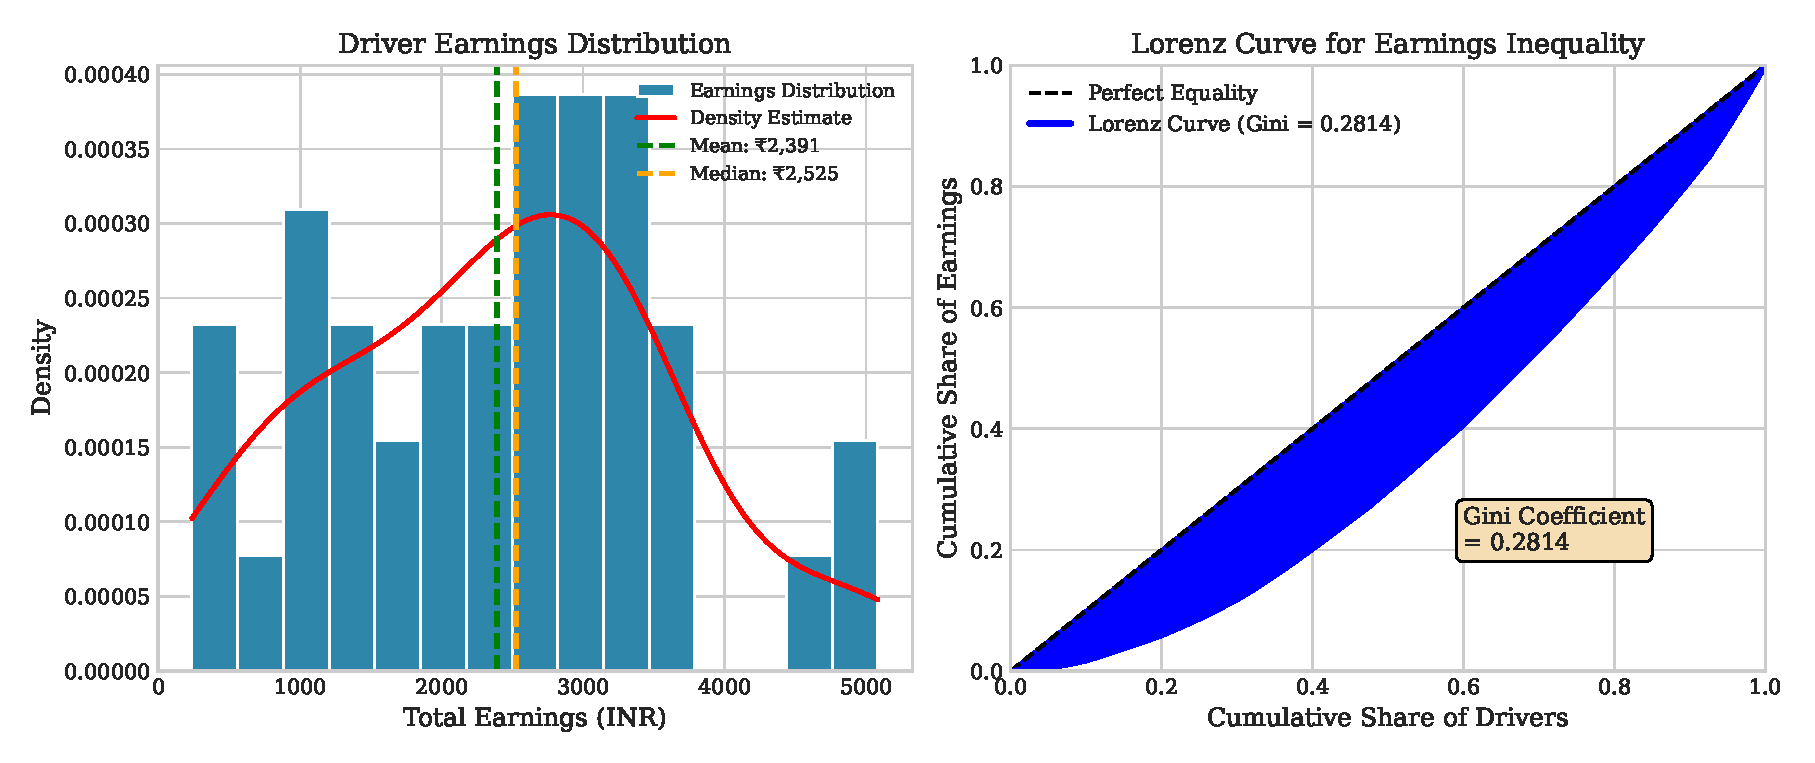
\includegraphics[width=\textwidth]{figures/fig3_earnings_distribution}
\caption{Driver earnings analysis: (Left) Histogram showing the distribution of total earnings per driver with kernel density estimate. (Right) Lorenz curve illustrating earnings inequality with Gini coefficient of 0.2814.}
\label{fig:earnings}
\end{figure}

The average earnings per trip was \rupee 303.08 with a median of \rupee 283.71. Drivers completed an average of 8.0 trips during the observation period.

\subsection{Trip Completion Analysis}
Table~\ref{tab:tripstatus} presents the trip status distribution.

\begin{table}[htbp]
\caption{Trip Status Distribution}
\label{tab:tripstatus}
\begin{center}
\begin{tabular}{lrr}
\toprule
\textbf{Status} & \textbf{Count} & \textbf{Percentage} \\
\midrule
Completed & 386 & 78.1\% \\
Rider Cancelled & 100 & 20.2\% \\
Driver Cancelled & 8 & 1.6\% \\
\midrule
\textbf{Total} & \textbf{494} & \textbf{100\%} \\
\bottomrule
\end{tabular}
\end{center}
\end{table}

The completion rate of 78.1\% is consistent with industry benchmarks. Notably, rider cancellations (20.2\%) significantly exceed driver cancellations (1.6\%), indicating good driver reliability.

Service type distribution shows UberGo as the dominant product (94.3\%), followed by UberX+ (4.3\%) and Intercity (1.0\%).

\subsection{Trip Distance and Fare Analysis}
Analysis of 386 completed trips with valid distance data reveals the statistics in Table~\ref{tab:distancefare}.

\begin{table}[htbp]
\caption{Distance and Fare Statistics}
\label{tab:distancefare}
\begin{center}
\begin{tabular}{lrr}
\toprule
\textbf{Metric} & \textbf{Distance (km)} & \textbf{Fare (\rupee)} \\
\midrule
Mean & 17.17 & 324.83 \\
Median & 14.70 & 272.14 \\
Std. Deviation & 15.08 & 233.07 \\
Minimum & 1.13 & 89.92 \\
Maximum & 188.77 & 2,672.84 \\
\bottomrule
\end{tabular}
\end{center}
\end{table}

The average fare per kilometer was \rupee 22.70 with a median of \rupee 19.57. Table~\ref{tab:distcat} shows fare patterns by distance category.

\begin{table}[htbp]
\caption{Analysis by Distance Category}
\label{tab:distcat}
\begin{center}
\begin{tabular}{lrrr}
\toprule
\textbf{Category} & \textbf{Trips} & \textbf{Avg Fare} & \textbf{\rupee/km} \\
\midrule
Short ($\leq$5 km) & 44 & 132.58 & 41.64 \\
Medium (5-15 km) & 153 & 230.29 & 23.93 \\
Long (15-25 km) & 119 & 334.37 & 17.29 \\
Very Long ($>$25 km) & 70 & 636.07 & 17.31 \\
\bottomrule
\end{tabular}
\end{center}
\end{table}

The decreasing fare per kilometer with increasing distance reflects the typical fare structure where the base fare has a higher impact on shorter trips.

\subsection{Fare-Distance Regression Model}
Linear regression analysis yields:
\begin{equation}
\text{Fare} = 14.64 \times \text{Distance} + 73.50
\end{equation}

The model statistics are:
\begin{itemize}
\item Pearson Correlation: $r = 0.9470$
\item Coefficient of Determination: $R^2 = 0.8968$
\item P-value: $1.80 \times 10^{-191}$
\end{itemize}

The high $R^2$ value indicates that distance explains 89.68\% of fare variance. The intercept of \rupee 73.50 represents the effective base fare, while the slope of \rupee 14.64/km represents the distance-based fare component.

Figure~\ref{fig:regression} visualizes the fare-distance relationship with the fitted regression line and 95\% confidence interval, demonstrating the strong linear relationship between these variables.

\begin{figure}[htbp]
\centering
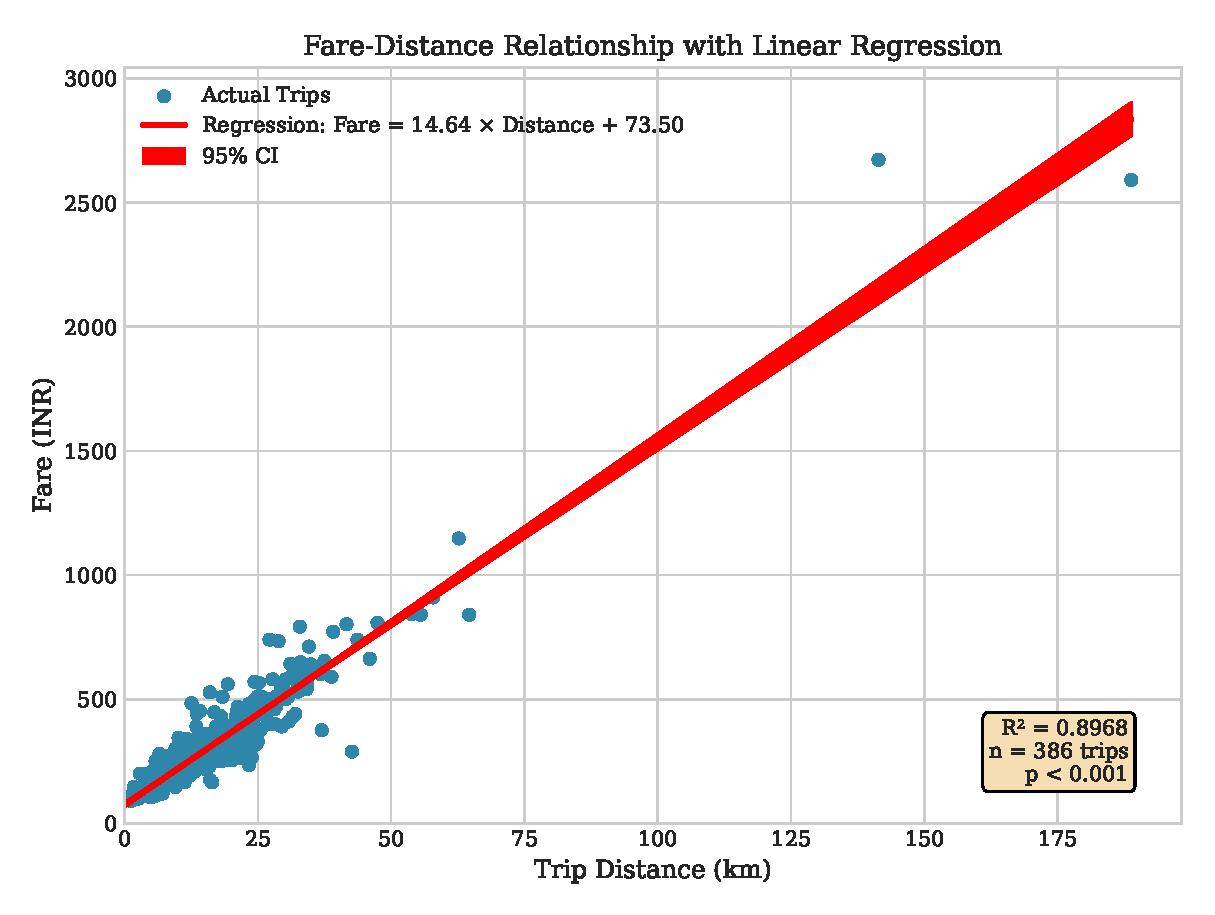
\includegraphics[width=0.9\textwidth]{figures/fig1_fare_distance_regression}
\caption{Scatter plot of fare versus trip distance with linear regression line. The model achieves $R^2 = 0.8968$, indicating that distance explains approximately 90\% of fare variance. Shaded region represents the 95\% confidence interval.}
\label{fig:regression}
\end{figure}

\subsection{Payment Mode Analysis}
Cash remains the predominant payment mode:
\begin{itemize}
\item Cash Trips: 286 (89.7\%)
\item Digital Trips: 33 (10.3\%)
\end{itemize}

Average fare for cash trips (\rupee 314.36) is significantly higher than digital trips (\rupee 162.55), suggesting that longer-distance trips tend to be paid in cash.

\subsection{Temporal Patterns}
Trip distribution across time periods shows relatively uniform demand:
\begin{itemize}
\item Morning (6AM-12PM): 147 trips (29.8\%)
\item Afternoon (12PM-6PM): 143 trips (28.9\%)
\item Evening (6PM-12AM): 146 trips (29.6\%)
\item Night (12AM-6AM): 58 trips (11.7\%)
\end{itemize}

Peak hours were identified as 21:00-22:00 (34 trips) and 11:00-12:00 (33 trips). Figure~\ref{fig:temporal} provides a detailed visualization of the hourly trip distribution.

\begin{figure}[htbp]
\centering
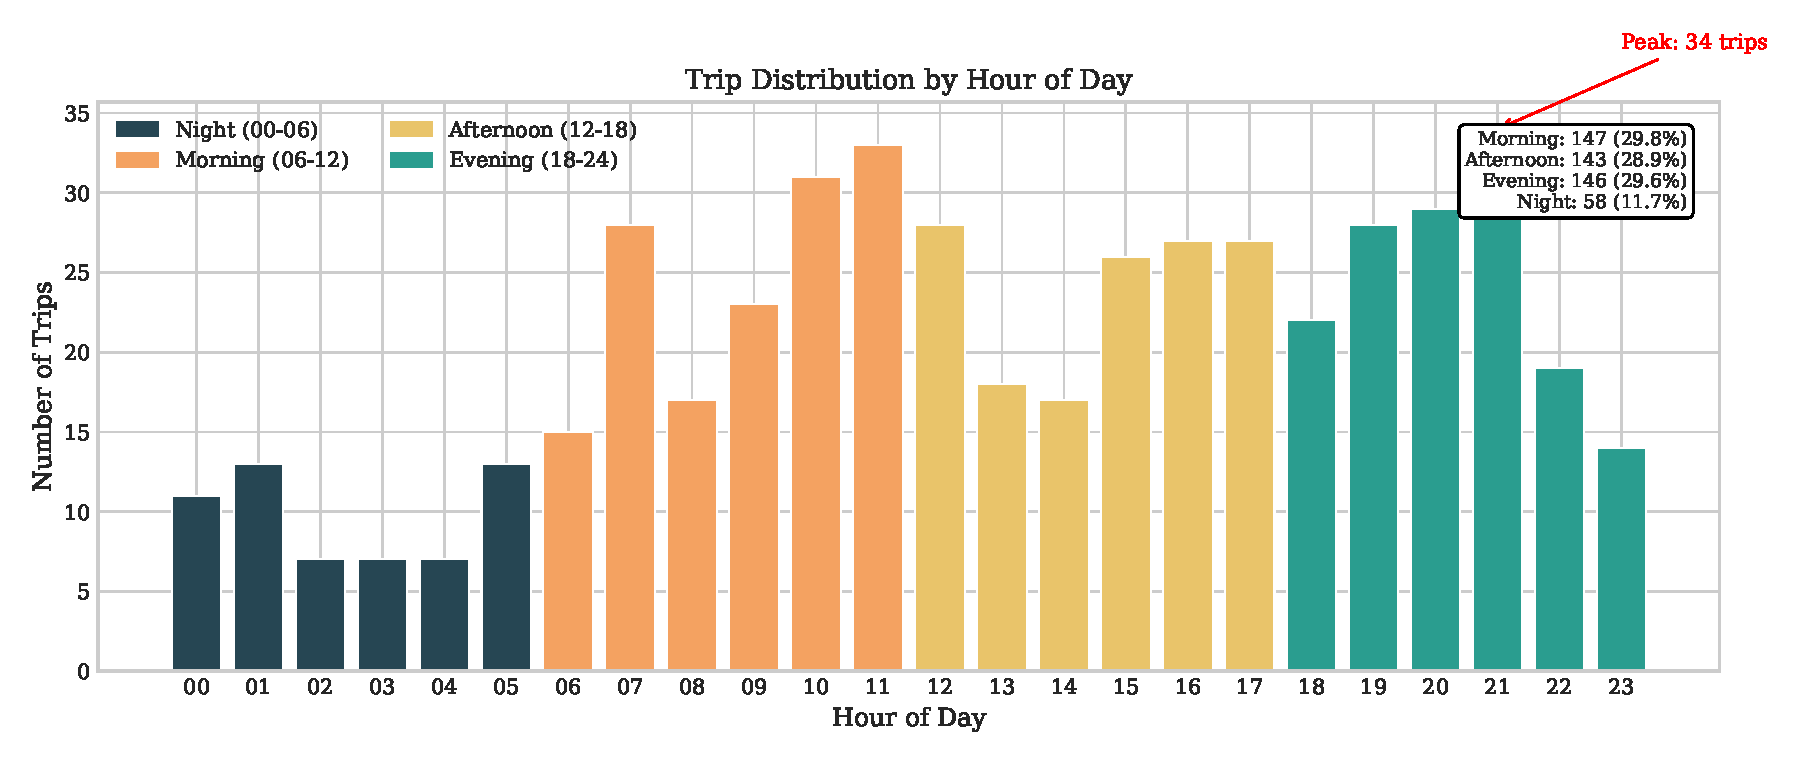
\includegraphics[width=\textwidth]{figures/fig4_temporal_patterns}
\caption{Hourly distribution of trip requests showing demand patterns across different time periods. Colors indicate time period categories: Night (00-06), Morning (06-12), Afternoon (12-18), and Evening (18-24). Peak demand occurs during evening hours.}
\label{fig:temporal}
\end{figure}

\subsection{Driver Performance Metrics}
Driver completion rates show significant variation:
\begin{itemize}
\item Mean Completion Rate: 78.6\%
\item High Performers ($\geq$80\%): 20 drivers (46.5\%)
\item Low Performers ($<$60\%): 5 drivers (11.6\%)
\end{itemize}

%
\section{Discussion}
%
\subsection{Implications for Fleet Operators}
Our findings have several practical implications:

\textbf{Revenue Optimization}: The dominance of base fare (89.2\%) suggests that increasing trip volume is more effective for revenue growth than relying on surge pricing. Fleet operators should focus on maximizing trip completion rates.

\textbf{Driver Management}: The moderate Gini coefficient (0.2814) indicates reasonably equitable earnings distribution. However, the presence of low-performing drivers (11.6\%) suggests opportunities for targeted training or support programs.

\textbf{Payment Infrastructure}: The high proportion of cash transactions (89.7\%) indicates potential for digital payment adoption initiatives, which could reduce cash handling costs and improve transaction efficiency.

\subsection{Fare Model Insights}
The regression model (Fare = 14.64 $\times$ Distance + 73.50) provides a transparent understanding of the fare structure:
\begin{itemize}
\item The base fare component (\rupee 73.50) covers fixed costs per trip
\item The per-kilometer rate (\rupee 14.64) reflects variable operational costs
\item The high explanatory power ($R^2 = 0.8968$) indicates consistent pricing
\end{itemize}

\subsection{Limitations}
This study has several limitations:
\begin{itemize}
\item The dataset represents a single fleet operator in one city
\item The observation period may not capture seasonal variations
\item External factors (fuel prices, traffic conditions) were not included
\item Driver-level characteristics were not available due to anonymization
\end{itemize}

\subsection{Future Research Directions}
Future work could extend this framework by:
\begin{itemize}
\item Incorporating machine learning models for demand prediction
\item Analyzing multi-city datasets for geographic comparison
\item Including driver behavior metrics for performance optimization
\item Developing real-time analytics dashboards for fleet operators
\end{itemize}

%
\section{Conclusion}
%
This paper presents a comprehensive financial analytics framework for ride-sharing fleet operations. Using real-world transaction data comprising 677 payment records and 494 trip activities, we derive actionable insights for fleet management.

Key findings include:
\begin{itemize}
\item Base fare contributes 89.2\% of total revenue, indicating the importance of trip volume over surge pricing
\item Driver earnings show moderate inequality (Gini = 0.2814) with mean earnings of \rupee 2,391.27
\item Trip completion rate of 78.1\% with rider cancellations (20.2\%) exceeding driver cancellations (1.6\%)
\item Linear regression explains 89.68\% of fare variance: Fare = 14.64 $\times$ Distance + 73.50
\item Cash payments dominate (89.7\%) with higher average fares than digital payments
\end{itemize}

The framework provides a template for fleet operators to analyze their operational data and make data-driven decisions. All analysis code is available for replication and extension.

\vspace{1cm}
\noindent
\textbf{Data Availability Statement}\\
The anonymized datasets and analysis code used in this study are publicly available at \url{https://github.com/ItsHarshitAg/financial_data_analysis}. All personally identifiable information has been removed from the datasets, including driver names, exact addresses, and original timestamps. Dates have been shifted by a fixed offset to preserve temporal patterns while protecting privacy.

\vspace{0.5cm}
\noindent
\textbf{Acknowledgements}\\
[Add acknowledgements here if applicable]

%
% ---- Bibliography ----
%
\begin{thebibliography}{10}
%

\bibitem{cramer2016}
Cramer, J., Krueger, A.B.: Disruptive change in the taxi business: The case of Uber.
American Economic Review 106(5), 177-182 (2016). \url{https://doi.org/10.1257/aer.p20161002}

\bibitem{chen2016}
Chen, M.K., Sheldon, M.: Dynamic pricing in a labor market: Surge pricing and flexible work on the Uber platform.
EC '16: Proceedings of the 2016 ACM Conference on Economics and Computation, pp. 455 (2016). \url{https://doi.org/10.1145/2940716.2940798}

\bibitem{hall2015}
Hall, J.V., Kendrick, C., Nosko, C.: The effects of Uber's surge pricing: A case study.
University of Chicago Booth School of Business (2015).

\bibitem{hall2018}
Hall, J.V., Krueger, A.B.: An analysis of the labor market for Uber's driver-partners in the United States.
ILR Review 71(3), 705-732 (2018). \url{https://doi.org/10.1177/0019793917717222}

\bibitem{cook2018}
Cook, C., Diamond, R., Hall, J.V., List, J.A., Oyer, P.: The gender earnings gap in the gig economy: Evidence from over a million rideshare drivers.
NBER Working Paper No. 24732 (2018). \url{https://doi.org/10.3386/w24732}

\bibitem{wang2019}
Wang, H., Yang, H.: Ridesourcing systems: A framework and review.
Transportation Research Part B: Methodological 129, 122-155 (2019). \url{https://doi.org/10.1016/j.trb.2019.07.009}

\bibitem{xu2020}
Xu, Z., Li, Z., Guan, Q., Zhang, D., Li, Q., Nan, J., Liu, C., Bian, W., Ye, J.: Large-scale order dispatch in on-demand ride-hailing platforms: A learning and planning approach.
KDD '18: Proceedings of the 24th ACM SIGKDD International Conference on Knowledge Discovery \& Data Mining, pp. 905-913 (2018). \url{https://doi.org/10.1145/3219819.3219824}

\bibitem{ke2017}
Ke, J., Zheng, H., Yang, H., Chen, X.M.: Short-term forecasting of passenger demand under on-demand ride services: A spatio-temporal deep learning approach.
Transportation Research Part C: Emerging Technologies 85, 591-608 (2017). \url{https://doi.org/10.1016/j.trc.2017.10.016}

\bibitem{gini1921}
Gini, C.: Measurement of inequality of incomes.
The Economic Journal 31(121), 124-126 (1921). \url{https://doi.org/10.2307/2223319}

\bibitem{mckinneyPandas}
McKinney, W.: Data structures for statistical computing in Python.
In: Proceedings of the 9th Python in Science Conference, pp. 56-61 (2010). \url{https://doi.org/10.25080/Majora-92bf1922-00a}

\end{thebibliography}

\end{document}
